\section{Problem Statement}%
\label{sec:problem_statement}

\subsection{Toroidal Grid}%
\label{sub:toroidal_grid}

As per AZsPCs\cite{zimmermann} specifications, the initial toroidal grid $O$ is defined as an $N\times N$ grid of unique tokens which ``wrap around'' the edges. A token is of the form $\bm{IJ}$, where $\bm{I}$ and $\bm{J}$ are alphabetic representations of the indices of the rows and columns respectively, of a token, \emph{within $O$},\footnote{This is important because after rearranging the tokens, the identity of the token depends on its position within $O$, and not the rearranged position} e.g., $AC$ corresponds to the token in row 1, column 3 of $O$, $DF$ corresponds to the row 4, column 6 of $O$, etc. \autoref{fig:toroidExample} shows $O$ for $N=4$. Tokens outside of the square grid represent tokens ``wrapping around'' the edges, resembling a toroidal surface as shown in \autoref{fig:wiki_toroid}.
\begin{figure}[htpb]
    \begin{subfigure}[t]{0.5\textwidth}
    \begin{center}
        \raisebox{0.4cm}{
        \includegraphics[width=0.7\textwidth]{images/Simple_Torus.pdf}}
    \caption{A Simple Toroid by Yassine Mrabet\cite{wiki_toroid}}
    \label{fig:wiki_toroid}
    \end{center}
    \end{subfigure}
    ~
    \begin{subfigure}[t]{0.5\textwidth}
    \begin{center}
    \toroidWarp{4}
    \caption{A $4\times 4$ \emph{intial} toroidal grid}%
    \label{fig:toroidExample}
    \end{center}
    \end{subfigure}
    \caption{Representations of a toroidal grid}
\end{figure}

\subsection{Evaluation Function}%
\label{sub:evaluation_function}

The goal of the challenge is to rearrange the tokens within $O$ to form a new grid $X$ that minimizes a loss function computed with the following procedure:
\begin{enumerate}
    \item For each unique pair of tokens (e.g., $[AA,BA]$ is equivalent to $[BA,AA]$, so $[BA,AA]$ is omitted), calculate the squared distance between them in $X$,
    \item Multiply each of these by the squared distance between the pair of tokens within $O$,
    \item Sum all of these products,
    \item Subtract a lower-bound corresponding to the value of $N$ (\autoref{sec:lower_bound_constants})
\end{enumerate}

\subsection{Distance Metric}%
\label{sub:distance_metric}
To evaluate the loss function, a distance metric between two tokens must be established, which necessitates a coordinate system. Here, \emph{the coordinate of a token is defined as the indices of the token within $X$} i.e., any token within row 5, column 3 of $X$, has coordinates $(5,3)$. Note that within $O$, coordinates, indices, and token representations are all equivalent.

 Let two two-dimensional coordinates be $s_1=(x_1,y_1)$ and $s_2=(x_2,y_2)$. The Euclidean distance $d_{euclid}$ is defined as,%
\begin{align}
    \label{eq:euclid}
    d_{euclid}(s_1,s_2)=\sqrt{(x_2-x_1)^2+(y_2-y_1)^2}=\sqrt{(\Delta_{euclid} x)^2+(\Delta_{euclid} y)^2}
\end{align}

On a toroidal surface however, $\Delta x$ and $\Delta y$ can each have 2 possible values. A one-dimensional toroidal surface of length $N$ is illustrated in \autoref{fig:2distanceexample}. The corresponding possible values for $\Delta x$ are as follows,%
\begin{align}
    \Delta_1(x)&=x_2-x_1\nonumber\\
    \Delta_2(x)&=(x_1-0)+(N-x_2)=x_1+N-x_2
    \label{eq:naiveToroidDistance}
\end{align}

\begin{figure}[htpb]
    \centering
    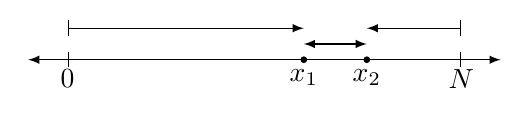
\begin{tikzpicture}
        \draw[latex-latex] (-3,0) -- (3,0);
        \draw[|-|] (-2.5,0) node[below] {$0$} -- (2.5,0) node[below] {$N$};
        %\draw[|-|] (-2.5,-0.5) -- node[below] {$N$} (2.5,-0.5);
        \filldraw (0.5,0) circle (1pt) node[below] {$x_1$};
        \filldraw (1.3,0) circle (1pt) node[below] {$x_2$};
        \draw[latex-latex] (0.5,0.2) -- (1.3,0.2);
        \draw[latex-|] (1.3,0.4) -- (2.5,0.4);
        \draw[|-latex] (-2.5,0.4) -- (0.5,0.4);
    \end{tikzpicture}
    \caption{A one-dimensional diagram of toroidal distance, with the two arrows representing two possible distances}%
    \label{fig:2distanceexample}
\end{figure}

To obtain a general equation that works when $x_1>x_2$:%
\begin{align}
    \Delta_1(x)&=\lvert x_2-x_1 \rvert\nonumber\\
    \Delta_2(x)&=\min{(x_1,x_2)}+N-\max{(x_1,x_2)}
    %\label{eq:absoluteToroidDistance}
\end{align}
where $\lvert a\rvert$ is the absolute value of $a$, $\min{(a,b)}$ and $\max{(a,b)}$ are defined as the minimum and maximum between the values of $a$ and $b$ respectively, that is,%
\begin{align}
        \min{(a,b)}=
        \begin{cases}
            a,&\text{if $a\leq b$}\\
            b,&\text{if $a>b$}
        \end{cases}\qquad
        \max{(a,b)}=
        \begin{cases}
            a,&\text{if $a\geq b$}\\
            b,&\text{if $a<b$}
        \end{cases}
\end{align}
$\min$ and $\max$ are used to determine the  ``left-most'' and the ``right-most'' coordinates.

One-dimensional toroidal distance is then defined as%
\begin{align}
    \Delta x=\min{(\Delta_1(x),\Delta_2(x))}
\end{align}

And in two dimensions, the toroidal distance and squared toroidal distance are%
\begin{align}
    d(s_1,s_2)&=\sqrt{(\Delta x)^2+(\Delta y)^2}\nonumber\\
    d^2(s_1,s_2)&=(\Delta x)^2+(\Delta y)^2
\end{align}
From now on, \emph{distance} refers to $d^2$.

For example, the distance between $s_1=(1,4),s_2=(2,1)$ and $N=5$ is calculated as follows:%
\begin{align}
    \Delta_1(x)&=\lvert 2-1\rvert=1\nonumber\\
    \Delta_2(x)&=\min{(1,2)}+5-\max{(1,2)}=1+5-2=4\nonumber\\
    \Delta_1(y)&=\lvert 1-4\rvert=3\nonumber\\
    \Delta_2(y)&=\min{(4,1)}+5-\max{(4,1)}=1+5-4=2\nonumber\\
    \Delta(x)&=\min{(1,4)}=1\nonumber\\
    \Delta(y)&=\min{(3,2)}=2\nonumber\\
    d^2(s_1,s_2)&=1^2+2^2=5
\end{align}

\subsection{Token Comparisons}%
\label{sub:token_comparisons}
\begin{figure}[htpb]
    \centering
    \begin{subfigure}[t]{0.5\textwidth}
    \begin{center}
    \nestedToroid{2}
    \end{center}
    \caption{}
    \label{fig:4dcomparison}
    \end{subfigure}%
    ~
    \begin{subfigure}[t]{0.5\textwidth}
    \begin{center}
    \twodcomparison{2}
    \end{center}
    \caption{}
    \label{fig:2dcomparison}
    \end{subfigure}

    \caption{Tensors $C(X)$ in the forms $C(X)_{i,j,k,l}$ and $C(X)_{m,n}$ respectively, representing comparison grids of an $N=2$ toroidal grid, where every element represents the distance between tokens $\bm{IJ}$ and $\bm{KL}$ within $X$. Shaded cells denote unique comparisons.}%
    \label{fig:comparisonGrids}
\end{figure}

In order to compute distances between all possible pairs, a corresponding representation is required, i.e., a 4-dimensional matrix (or tensor) with elements being distances between \emph{source} tokens (first 2 dimensions) and \emph{target} tokens (next 2 dimensions). An example of the structure of the comparison for an $N=2$ grid is shown in \autoref{fig:4dcomparison}.

\begin{figure}[htpb]
    \centering
    \flatten{3}
    \caption{Matrix-flattening}%
    \label{fig:matrix_flattening}
\end{figure}
The dimensionality of the grid can be reduced from a tensor into a matrix, to reduce complexity (e.g., number of $\Sigma$s in \ref{sub:loss_function_as_matrix_multiplications}) by applying the matrix-flattening scheme in \autoref{fig:matrix_flattening} twice, on the source and target dimensions, reducing $C(X)$ from $N\times N\times N\times N$ to $N^2\times N^2$. Elements within the 4-dimensional tensor are of form $C(X)_{i,j,k,l}$, whereas the 2-dimensional elements are of form $C(X)_{m,n}$. To do this conversion,%
\begin{align}
    m=(i-1)\times N+j &\implies m\div N=i-1 \text{ remainder } j\nonumber\\
    n=(k-1)\times N+l &\implies n\div N=j-1 \text{ remainder } l
    \label{eq:flattening_scheme}
\end{align}
\autoref{eq:flattening_scheme} can be understood by realizing that $A_{2,3}$ (\autoref{fig:matrix_flattening}) is offset by $(2-1)$ groups of 3 and an additional 3 after flattening.

Note that both $C(X)_{i,j,k,l}$ and $C(X)_{m,n}$ represent the distance between tokens $\bm{IJ}$ and $\bm{KL}$ within $X$ as defined within \autoref{sub:distance_metric}, the difference lies only within their dimensionality. The two-dimensional representation of \autoref{fig:4dcomparison} is shown in \autoref{fig:2dcomparison}.

From now on, let $C(X)$ refer to the two dimensional comparison grid. Examples are shown in \autoref{fig:comparisonExample}.

\begin{figure}[htpb]
    \begin{subfigure}[b]{0.5\textwidth}
    \begin{center}
\drawGrid{2}{{AA,AB,BA,BB}}
    \end{center}
    \caption{$O$}
    \end{subfigure}%
    \begin{subfigure}[b]{0.5\textwidth}
    \begin{center}
        \begin{align*}
            \begin{blockarray}{ccccc}
            &AA & AB & BA & BB \\
            \begin{block}{c[cccc]}
                AA&0&1&1&2\\
                AB&1&0&2&1\\
                BA&1&2&0&1\\
                BB&2&1&1&0\\
            \end{block}
            \end{blockarray}
        \end{align*}
    \end{center}
    %\vspace{-\baselineskip}
    \caption{$C(O)$}
    \label{fig:c_o}
    \end{subfigure}
    \begin{subfigure}[b]{0.5\textwidth}
    \begin{center}
\drawGrid{2}{{AA,AB,BB,BA}}
    \end{center}
    \caption{An example toroidal grid $X$}
    \end{subfigure}%
    \begin{subfigure}[b]{0.5\textwidth}
    \begin{center}
        \begin{align*}
            \begin{blockarray}{ccccc}
            &AA & AB & BA & BB \\
            \begin{block}{c[cccc]}
                AA&0&1&2&1\\
                AB&1&0&1&2\\
                BA&2&1&0&1\\
                BB&1&2&1&0\\
            \end{block}
            \end{blockarray}
        \end{align*}
    \end{center}
    \vspace{-\baselineskip}
    \caption{$C(X)$}
    \end{subfigure}
    \caption{Example toroidal grids and comparison grids}
    \label{fig:comparisonExample}
\end{figure}

\subsection{Loss Function in Matrix Form}%
\label{sub:loss_function_as_matrix_multiplications}
The computation of products of only unique comparisons is greatly simplified due to the 2-dimensional representation (\autoref{fig:2dcomparison}) of $C(X)$, which is symmetric along the main diagonal i.e., unique comparisons (shaded cells) along the upper triangle are mirrored along the lower triangle i.e., %
$\begin{smallmatrix}
    AA\\ AB
\end{smallmatrix}
$ is mirrored by
$
\begin{smallmatrix}
    AB\\ AA
\end{smallmatrix}
$. Also, the elements of $C(O)$ and $C(X)$ are zero-valued along the diagonal (i.e., not contributing to the loss function) due to the distance between a point and itself being $0$. Therefore, to calculate the loss function a simple factor of $\frac{1}{2}$ can be added, and the loss of $X$, $L(X)$ can be written as:
\begin{align}
    L(X)&=\frac{1}{2}\sum_m^{N^2}\sum_n^{N^2}C(X)_{m,n}C(O)_{m,n}-c\nonumber\\
        &=\frac{1}{2}\sum_m^{N^2}\sum_n^{N^2}(C(X)\odot C(O))_{m,n}-c
\end{align}
Where $(\odot)$ denotes element-wise multiplication, that is\footnote{every element within $C$ is equal to the product of the elements of $A$ and $B$ within that position}
\begin{align}
    C=A\odot B \implies C_{i,j}=A_{i,j}B_{i,j}\;\forall i,j
\end{align}

The loss function for \autoref{fig:comparisonExample} is computed as follows:
\begin{align}
    L(X)&=\frac{1}{2}\sum_m^{N^2}\sum_n^{N^2}(C(X)\odot C(O))_{m,n}-c\nonumber\\
        &=\frac{1}{2}\sum_m^{N^2}\sum_n^{N^2}
        \left(\begin{bmatrix}
        0&1&2&1\\
        1&0&1&2\\
        2&1&0&1\\
        1&2&1&0
    \end{bmatrix}\odot
    \begin{bmatrix}
        0&1&1&2\\
        1&0&2&1\\
        1&2&0&1\\
        2&1&1&0\\
    \end{bmatrix}\right)_{m,n}-c\nonumber\\
        &=\frac{1}{2}\sum_m^{N^2}\sum_n^{N^2}
\begin{bmatrix}
    0&1&2&2\\
    1&0&2&2\\
    2&2&0&1\\
    2&2&1&0
\end{bmatrix}_{m,n}
        -c\nonumber\\
        &=\frac{1}{2}\cdot 20-c\nonumber\\
        &=10-c
        \label{eq:discrete_example}
\end{align}
